%
% Source : https://github.com/Seb75000/LaTeXTemplate
% Licence Apache-2.0
%
% Le fichier principal, qui appelle les autres. Ici utilisé avec des packages permettant de faire la mise en page qui me convenait.
% Compilation OK avec Overleaf, que je recommande chaudement dans sa version payante :
% - paiement au mois (9,60€ pour 1 mois) :
%   - durée de compilation plus élevée, les timeouts de la version gratuite sont chiants quand le doc devient un peu gros
%   - Support du travail collaboratif (faites vous relire !!!)
%   - synchro avec Github
% - Versioning
% - Support de tous les packages que j'ai ajoutés, et contournement des problèmes qu'ils peuvent poser
%
% Pull requests bienvenues, surtout pour la page de couverture qui est clairement bancale !
% Faites en bon usage, et si ça vous sert, un petit message sur github via une issue serait très apprécié !


\documentclass{report}

% Language setting
\usepackage[french]{babel}

% Set page size and margins
\usepackage[a4paper,top=2cm,bottom=2cm,left=3cm,right=3cm,marginparwidth=1.75cm]{geometry}

% Useful packages
%\usepackage{amsmath}
\usepackage[pages=some]{background}
\usepackage{float} % Place les images à l'endroit désiré
\usepackage[bottom]{footmisc}
\usepackage{graphicx}
\usepackage[colorlinks=true, allcolors=blue]{hyperref}
\usepackage{textpos}
\usepackage[utf8]{inputenc}
\usepackage{shadethm}
\usepackage{tcolorbox}
\usepackage{enumitem}
\usepackage{pdfpages}

% Gestion dest listings et du YAML
    \usepackage{courier} % Fonte Courier pour les extraits de code
    \usepackage{listings} % Et de quoi insérer des listings avec des options cools
    \newcommand\YAMLcolonstyle{\color{red}\mdseries}
    \newcommand\YAMLkeystyle{\color{black}\bfseries}
    \newcommand\YAMLvaluestyle{\color{blue}\mdseries}
    
    \makeatletter
    
    % here is a macro expanding to the name of the language
    % (handy if you decide to change it further down the road)
    \newcommand\language@yaml{yaml}
    
    \expandafter\expandafter\expandafter\lstdefinelanguage
    \expandafter{\language@yaml}
    {
      keywords={true,false,null,y,n},
      keywordstyle=\color{darkgray}\bfseries,
      basicstyle=\YAMLkeystyle,                                 % assuming a key comes first
      sensitive=false,
      comment=[l]{\#},
      morecomment=[s]{/*}{*/},
      commentstyle=\color{purple}\ttfamily,
      stringstyle=\YAMLvaluestyle\ttfamily,
      moredelim=[l][\color{orange}]{\&},
      moredelim=[l][\color{magenta}]{*},
      moredelim=**[il][\YAMLcolonstyle{:}\YAMLvaluestyle]{:},   % switch to value style at :
      morestring=[b]',
      morestring=[b]",
      literate =    {---}{{\ProcessThreeDashes}}3
                    {>}{{\textcolor{red}\textgreater}}1     
                    {|}{{\textcolor{red}\textbar}}1 
                    {\ -\ }{{\mdseries\ -\ }}3,
    }
    
    % switch to key style at EOL
    \lst@AddToHook{EveryLine}{\ifx\lst@language\language@yaml\YAMLkeystyle\fi}
    \makeatother
    
    \newcommand\ProcessThreeDashes{\llap{\color{cyan}\mdseries-{-}-}}




% Permet de mettre le numéro de page en bas comme pour un document de classe article, mais pour un book
    \usepackage{fancyhdr}
    \pagestyle{fancy}
    \fancyhf{} % Clear all header and footer fields
    \fancyfoot[C]{\thepage} % Center the page number in the footer
    \renewcommand{\headrulewidth}{0pt} % Remove the header rule

% Utiliser biblatex avec le style verbose-note
    \usepackage[style=verbose-note,defernumbers=false,sorting=none,backend=biber]{biblatex}
    % \usepackage[style=numeric,backend=biber,sorting=none]{biblatex}
    % \usepackage[style=verbose-note,backend=biber,sorting=none]{biblatex}
    \addbibresource{bibliographie.bib}

% Redéfinir l'underscore pour qu'il soit interprété comme un caractère normal
    \chardef\_=`_


\title{Titre du mémoire}
\author{Nom de l'auteur}

\begin{document}

% Attention aux modifs dans cette page, elle est plutôt buggée. Bien versionner les modifications et compiler à chaque modif :)
% Vraiment preneur d'une page mieux foutue si vous trouvez comment mieux faire !

\begin{titlepage}
%\BgThispage
\begin{textblock}{3.5}[0.5,0.5](0.5,0.5)
	
\includegraphics[width=4cm]{Images/00/LogoEsiea.png}\\[4cm]
  \end{textblock}
  
\begin{textblock}{2}[0.5,0.5](9.7,0.15)
 
\includegraphics[width=3cm]{Images/00/lorem.png}\\[2cm]   
  \end{textblock}
  
%\bigskip
\bigskip
\begin{center}

\vspace{1cm}
{\large \textbf{MÉMOIRE DE THÈSE PROFESSIONNELLE}}\\[0.6cm]

{ \large{Mastère Spécialisé\\[0.2cm]
Sécurité de l'Information et des Systèmes\\[0.2cm]
de l'ESIEA\\[0.2cm]
(MS-SIS)}}
\\[1cm]
% Title
\rule{\linewidth}{0.5mm} \\[0.5cm]
{ \huge \bfseries Objet du mémoire en question
 \\[0.5cm] }
\large Un chouette sous-titre 
\rule{\linewidth}{0.5mm} \\[1.5cm]

% Authors and supervisor
\noindent

\begin{textblock}{4}[0.5,0.5](1.5,0.5)
    {\Large \emph{Auteur :}}\\[0.3cm]
    {\large Vous}
\end{textblock}
  
\begin{textblock}{4}[0.5,0.5](8.7,0.5)
    {\Large \emph{Tuteur de stage :}}\\[0.3cm]
    {\large Pas vous}
\end{textblock}

%\\[4cm]
\vspace{4cm}

{\Large \emph{Composition du jury}}\\[0.8cm]



% {\Large  \emph{Class:}}\\[0.3cm]
% {\large 2\textsuperscript{nd}~ year INFO/TEL} \\[1cm]

\vspace{7cm}
% Bottom of the page

{Soutenance : 1970-01-01}
\end{center}

\end{titlepage}
%\maketitle
\section*{Remerciements}


\vspace{2cm}
\par 
Mon chien, mon chat, mon cochon d'inde

\bigskip
Ma famille

\bigskip
Mon réalisateur

\chapter*{Résumé}

\par
Lorem ipsum dolor sit amet, consectetur adipiscing elit, sed do eiusmod tempor incididunt ut labore et dolore magna aliqua. Ut enim ad minim veniam, quis nostrud exercitation ullamco laboris nisi ut aliquip ex ea commodo consequat. Duis aute irure dolor in reprehenderit in voluptate velit esse cillum dolore eu fugiat nulla pariatur. Excepteur sint occaecat cupidatat non proident, sunt in culpa qui officia deserunt mollit anim id est laborum.

\medskip
 \textbf{Mots clés} : Toto, tata, titi, tutu

\section*{Executive summary}
Lorem ipsum dolor, but in english, sit amet, consectetur adipiscing elit, sed do eiusmod tempor incididunt ut labore et dolore magna aliqua. Ut enim ad minim veniam, quis nostrud exercitation ullamco laboris nisi ut aliquip ex ea commodo consequat. Duis aute irure dolor in reprehenderit in voluptate velit esse cillum dolore eu fugiat nulla pariatur. Excepteur sint occaecat cupidatat non proident, sunt in culpa qui officia deserunt mollit anim id est laborum.


\medskip
\textbf{Keywords} : Toto, tata, titi, tutu

% La table des matières.
\tableofcontents

\chapter*{Introduction}
\textit{Lorem ipsum} (en italique) \footcite{loremIpsum} (ici une note de bas de page, qui se répercutera dans la bibliographie si et seulement si elle est utilisée. Elle doit être présente dans sample.bib) \textbf{dolor sit amet} (ou en gras), consectetur adipiscing elit, sed do eiusmod tempor incididunt ut labore et dolore magna aliqua.
\bigskip
Ut enim ad minim veniam, quis nostrud exercitation ullamco laboris nisi ut aliquip ex ea commodo consequat. Duis aute irure dolor in reprehenderit in voluptate velit esse cillum dolore eu fugiat nulla pariatur. Excepteur sint occaecat cupidatat non proident, sunt in culpa qui officia deserunt mollit anim id est laborum.

\medskip
blabla bla blabla.

\section*{Section 1}
Lorem ipsum dolor sit amet, consectetur adipiscing elit, sed do eiusmod tempor incididunt ut labore et dolore magna aliqua. Ut enim ad minim veniam, quis nostrud exercitation ullamco laboris nisi ut aliquip ex ea commodo consequat. Duis aute irure dolor in reprehenderit in voluptate velit esse cillum dolore eu fugiat nulla pariatur. Excepteur sint occaecat cupidatat non proident, sunt in culpa qui officia deserunt mollit anim id est laborum.

\begin{itemize}
    \item Element1 : blabla
    \item Element2 : blablabla
    \item Element3 : bleble
\end{itemize}


\section*{Une première section}
Lorem ipsum dolor sit amet, consectetur adipiscing elit, sed do eiusmod tempor incididunt ut labore et dolore magna aliqua. Ut enim ad minim veniam, quis nostrud exercitation ullamco laboris nisi ut aliquip ex ea commodo consequat. Duis aute irure dolor in reprehenderit in voluptate velit esse cillum dolore eu fugiat nulla pariatur. Excepteur sint occaecat cupidatat non proident, sunt in culpa qui officia deserunt mollit anim id est laborum.

\section*{Une deuxième section}

Lorem ipsum dolor sit amet, consectetur adipiscing elit, sed do eiusmod tempor incididunt ut labore et dolore magna aliqua. Ut enim ad minim veniam, quis nostrud exercitation ullamco laboris nisi ut aliquip ex ea commodo consequat. Duis aute irure dolor in reprehenderit in voluptate velit esse cillum dolore eu fugiat nulla pariatur. Excepteur sint occaecat cupidatat non proident, sunt in culpa qui officia deserunt mollit anim id est laborum.
Lorem ipsum dolor sit amet, consectetur adipiscing elit, sed do eiusmod tempor incididunt ut labore et dolore magna aliqua. Ut enim ad minim veniam, quis nostrud exercitation ullamco laboris nisi ut aliquip ex ea commodo consequat. Duis aute irure dolor in reprehenderit in voluptate velit esse cillum dolore eu fugiat nulla pariatur. Excepteur sint occaecat cupidatat non proident, sunt in culpa qui officia deserunt mollit anim id est laborum.

\section*{Une troisième section}
Lorem ipsum dolor sit amet, consectetur adipiscing elit, sed do eiusmod tempor incididunt ut labore et dolore magna aliqua. Ut enim ad minim veniam, quis nostrud exercitation ullamco laboris nisi ut aliquip ex ea commodo consequat. Duis aute irure dolor in reprehenderit in voluptate velit esse cillum dolore eu fugiat nulla pariatur. Excepteur sint occaecat cupidatat non proident, sunt in culpa qui officia deserunt mollit anim id est laborum.


\bigskip
\bigskip

\rule{\linewidth}{0.5mm} \\[0.5cm]

Petite conclusion de cette intro, ouverture vers le 1er chapitre

\begin{center}
\begin{tcolorbox}[colback=gray!10,
                  colframe=gray!50,
                  width=0.9\textwidth,
                  title=Titre de l'encart
                 ]
Un petit mot doux ici
Lorem ipsum dolor sit amet, consectetur adipiscing elit, sed do eiusmod tempor incididunt ut labore et dolore magna aliqua. Ut enim ad minim veniam, quis nostrud exercitation ullamco laboris nisi ut aliquip ex ea commodo consequat. Duis aute irure dolor in reprehenderit in voluptate velit esse cillum dolore eu fugiat nulla pariatur. Excepteur sint occaecat cupidatat non proident, sunt in culpa qui officia deserunt mollit anim id est laborum.
\end{tcolorbox}
\end{center}

\chapter{1er chapitre}

\section*{Introduction du 1er chapitre}

Le stage s'est effectué...

Lorem ipsum dolor sit amet, consectetur adipiscing elit, sed do eiusmod tempor incididunt ut labore et dolore magna aliqua. Ut enim ad minim veniam, quis nostrud exercitation ullamco laboris nisi ut aliquip ex ea commodo consequat. Duis aute irure dolor in reprehenderit in voluptate velit esse cillum dolore eu fugiat nulla pariatur. Excepteur sint occaecat cupidatat non proident, sunt in culpa qui officia deserunt mollit anim id est laborum.

\section{Section 1.1}

bla.
Avec un petit schéma, c'est toujours mieux !
\begin{figure}[H]
    \centering
    
\includegraphics[width=0.45\linewidth]{Images/10/lorem.png}
    \caption{Schéma lorem}
    \label{fig:LoremLabel}
\end{figure}

\section{Section 1.2}
Bla bla, mais pour la section 1.2 

\subsection{Et voici une subsection 1.2.1}

Les sous-sections découpent le propos 
    
\subsection{subsection 1.2.2}

lorem ipsum truc

\subsection{subsection 1.2.3}

Tu as compris l'idée


\medskip
Lorem ipsum dolor sit amet, consectetur adipiscing elit, sed do eiusmod tempor incididunt ut labore et dolore magna aliqua. Ut enim ad minim veniam, quis nostrud exercitation ullamco laboris nisi ut aliquip ex ea commodo consequat. Duis aute irure dolor in reprehenderit in voluptate velit esse cillum dolore eu fugiat nulla pariatur. Excepteur sint occaecat cupidatat non proident, sunt in culpa qui officia deserunt mollit anim id est laborum.
\section{Section 1.3}

\subsection{Subsection 1.3.1}
blabla
\subsection{Subsection 1.3.2}



\chapter{2e chapitre}

\section*{Introduction du 2e chapitre}

Lorem ipsum dolor sit amet, consectetur adipiscing elit, sed do eiusmod tempor incididunt ut labore et dolore magna aliqua. Ut enim ad minim veniam, quis nostrud exercitation ullamco laboris nisi ut aliquip ex ea commodo consequat. Duis aute irure dolor in reprehenderit in voluptate velit esse cillum dolore eu fugiat nulla pariatur. Excepteur sint occaecat cupidatat non proident, sunt in culpa qui officia deserunt mollit anim id est laborum.

\section{Section 2.1}

bla.
Avec un petit schéma, c'est toujours mieux !
\begin{figure}[H]
    \centering
    
\includegraphics[width=0.45\linewidth]{Images/10/lorem.png}
    \caption{Schéma lorem}
    \label{fig:LoremLabel}
\end{figure}

\section{Section 2.2}
Bla bla, mais pour la section 2.2 

\subsection{Et voici une subsection 2.2.1}

Les sous-sections découpent le propos 
    
\subsection{subsection 2.2.2}

lorem ipsum truc

\subsection{subsection 2.2.3}

Tu as compris l'idée


\medskip
Lorem ipsum dolor sit amet, consectetur adipiscing elit, sed do eiusmod tempor incididunt ut labore et dolore magna aliqua. Ut enim ad minim veniam, quis nostrud exercitation ullamco laboris nisi ut aliquip ex ea commodo consequat. Duis aute irure dolor in reprehenderit in voluptate velit esse cillum dolore eu fugiat nulla pariatur. Excepteur sint occaecat cupidatat non proident, sunt in culpa qui officia deserunt mollit anim id est laborum.
\section{Section 1.3}

\subsection{Subsection 2.3.1}
blabla
\subsection{Subsection 2.3.2}



\chapter{3e chapitre}

\section*{Introduction du 3e chapitre}

Lorem ipsum dolor sit amet, consectetur adipiscing elit, sed do eiusmod tempor incididunt ut labore et dolore magna aliqua. Ut enim ad minim veniam, quis nostrud exercitation ullamco laboris nisi ut aliquip ex ea commodo consequat. Duis aute irure dolor in reprehenderit in voluptate velit esse cillum dolore eu fugiat nulla pariatur. Excepteur sint occaecat cupidatat non proident, sunt in culpa qui officia deserunt mollit anim id est laborum.

\section{Section 3.1}

bla.
Avec un petit schéma, c'est toujours mieux !
\begin{figure}[H]
    \centering
    
\includegraphics[width=0.45\linewidth]{Images/30/lorem.png}
    \caption{Schéma lorem}
    \label{fig:LoremLabel}
\end{figure}

\section{Section 3.2}
Bla bla, mais pour la section 3.2 

\subsection{Et voici une subsection 3.2.1}

Les sous-sections découpent le propos 
    
\subsection{subsection 3.2.2}

lorem ipsum truc

\subsection{subsection 3.2.3}

Tu as compris l'idée


\medskip
Lorem ipsum dolor sit amet, consectetur adipiscing elit, sed do eiusmod tempor incididunt ut labore et dolore magna aliqua. Ut enim ad minim veniam, quis nostrud exercitation ullamco laboris nisi ut aliquip ex ea commodo consequat. Duis aute irure dolor in reprehenderit in voluptate velit esse cillum dolore eu fugiat nulla pariatur. Excepteur sint occaecat cupidatat non proident, sunt in culpa qui officia deserunt mollit anim id est laborum.
\section{Section 3.3}

\subsection{Subsection 3.3.1}
blabla
\subsection{Subsection 3.3.2}



\chapter*{Acronymes}
\addcontentsline{toc}{chapter}{Acronymes}

%\addcontentsline{toc}{section}{Acronymes génériques}
%\vspace{1cm}
\section*{Acronymes utilisés dans ce document}

\begin{description}[leftmargin=2.4cm,style=nextline]
    \item [AD] Active Directory
    \item [AI (ou IA)] Artificial Intelligence - Intelligence Artificielle
    \item [GPO] Group Policy Object
    \item [TTP] Tactiques, Techniques et Procédures
    \item [WMI] Windows Management Instrumentation
\end{description}


% Ici la bibliographie : toutes les notes de bas de page dans le corps du texte sont renvoyées dans cette biblio. Elles doivent être présentes dans bibliographie.bib. Si une note est dans bibliographie.bib mais pas utilisée dans le corps de texte, elle n'apparaîtra pas dans la bibliographie.
% Attention, la bibliographie est un peu chiante à faire dans la partie état de l'art, donc il existe des outils pour faire une partie du job : vous visitez un site qui vous intéresse pour le mémoire, et vous ajoutez automatiquement les données (page, titre, date...) dans un fichier utile. Je n'ai pas utilisé mais j'aurais dû. Mais du coup, démerdez vous pour trouver le bon outil :)
\printbibliography

% Cette annexe est sensée contenir du code, mais c'est tout buggé. Donc j'ai privilégié importer une annexe en PDF (cf plus bas)
%\chapter*{Annexe 1}

\begin{lstlisting}[language=python, basicstyle=\ttfamily\small, frame=single]

# Importation des modules necessaires
import random
import time

# Définition d'une fonction d'exemple
def lorem_ipsum_function(param1, param2):
    """
    Cette fonction est un exemple de code lorem ipsum.
    Elle ne fait rien de particulier mais illustre une structure de code.
    """
    result = param1 + param2
    for i in range(10):
        result += random.randint(1, 10)
        time.sleep(0.1)  # Simule un temps de traitement

    if result % 2 == 0:
        print("Le résultat est pair.")
    else:
        print("Le résultat est impair.")

    return result

# Définition d'une classe d'exemple
class LoremIpsumClass:
    def __init__(self, value):
        self.value = value

    def process_value(self):
        self.value *= 2
        print(f"La valeur traitée est : {self.value}")

    def display_value(self):
        print(f"La valeur actuelle est : {self.value}")

# Utilisation de la fonction et de la classe
if __name__ == "__main__":
    # Appel de la fonction
    result = lorem_ipsum_function(5, 10)
    print(f"Résultat de la fonction : {result}")

    # Création d'une instance de la classe
    lorem_instance = LoremIpsumClass(20)
    lorem_instance.display_value()
    lorem_instance.process_value()
    lorem_instance.display_value()

    # Boucle d'exemple
    for i in range(5):
        print(f"Itération {i} : {random.choice(['foo', 'bar', 'baz'])}")

    # Condition d'exemple
    if result > 50:
        print("Le résultat est supérieur à 50.")
    else:
        print("Le résultat est inférieur ou égal à 50.")

\end{lstlisting}



\chapter*{Annexe}

Ici vient une annexe pour mettre des éléments tiers pour le mémoire.
% ici en PDF
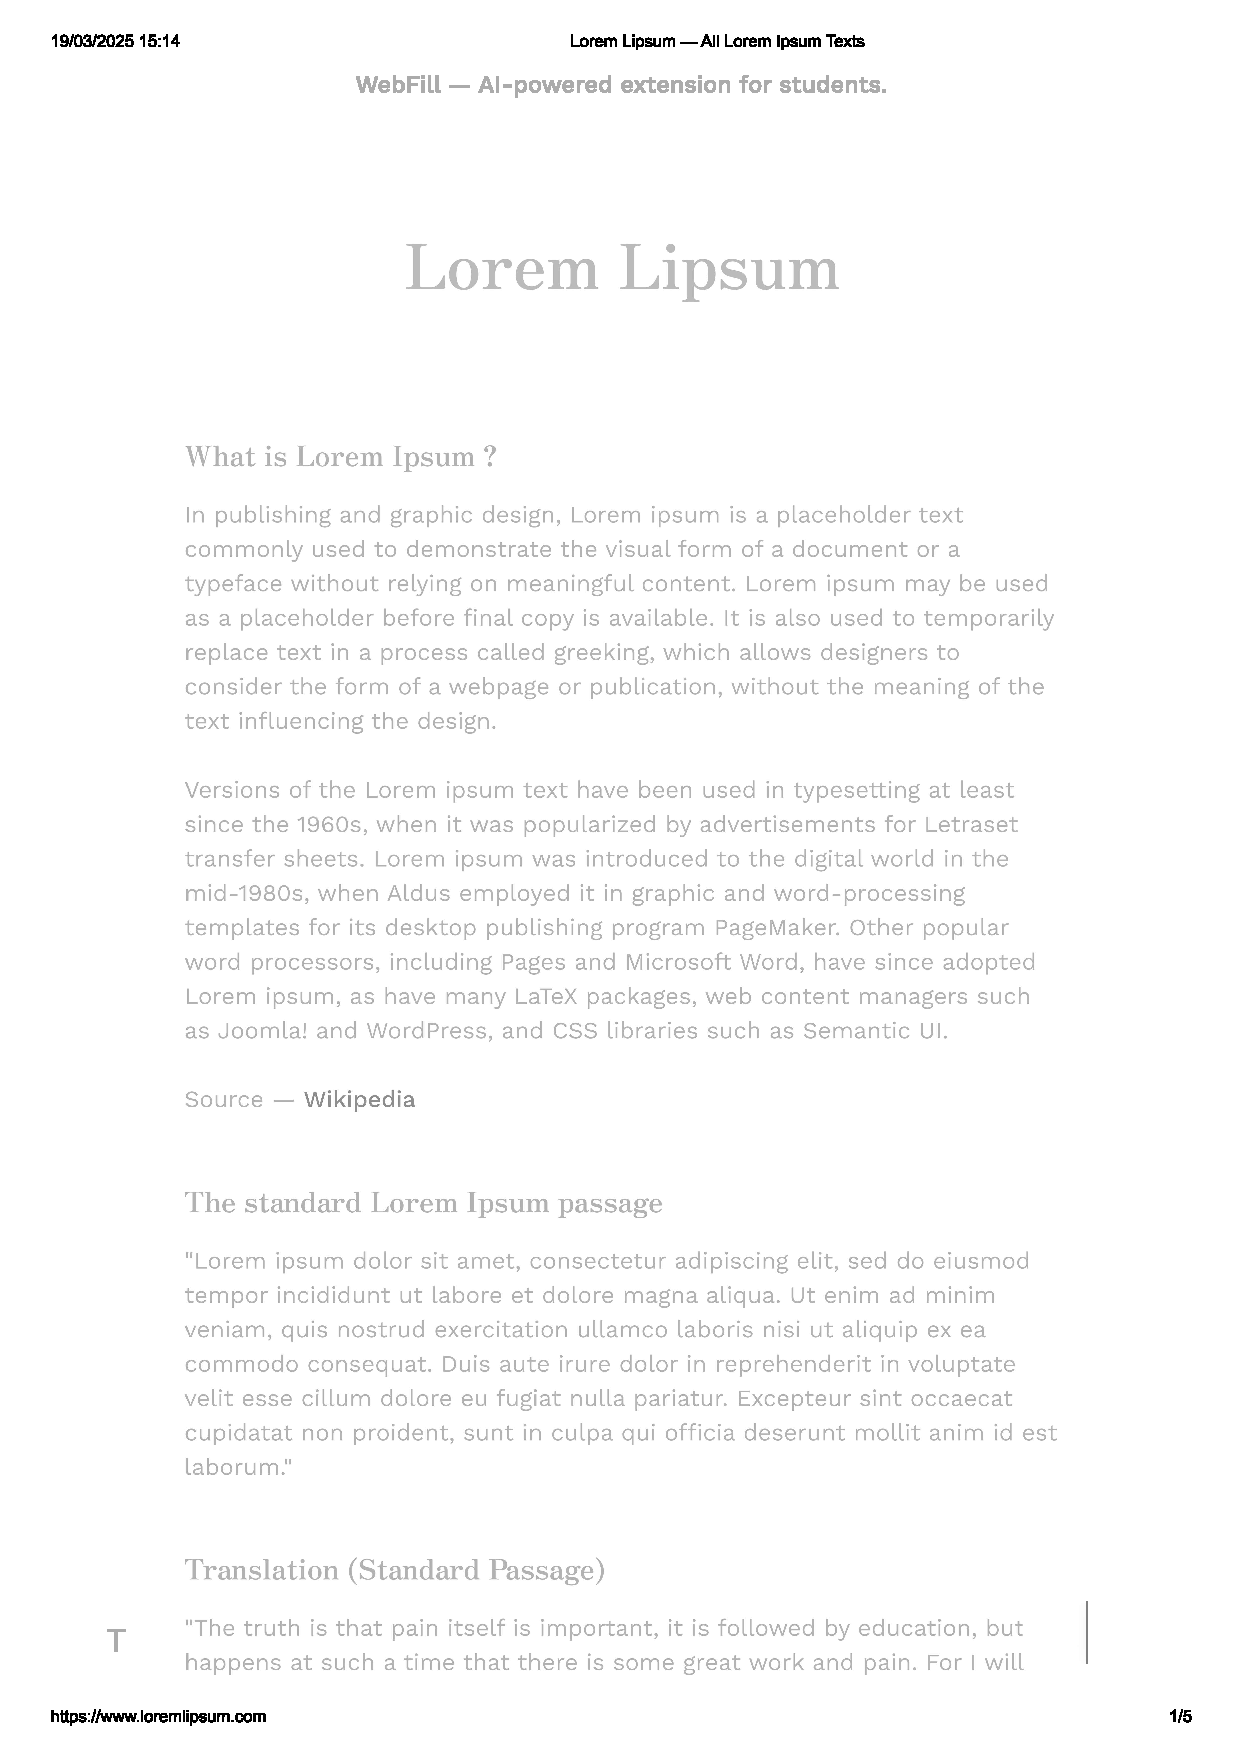
\includepdf[pages=-]{Include/lorem.pdf}

\end{document}